\section{系统设计}

\subsection{总体设计}

\subsubsection{功能设计}

\begin{figure}[thbp!]
	\centering
	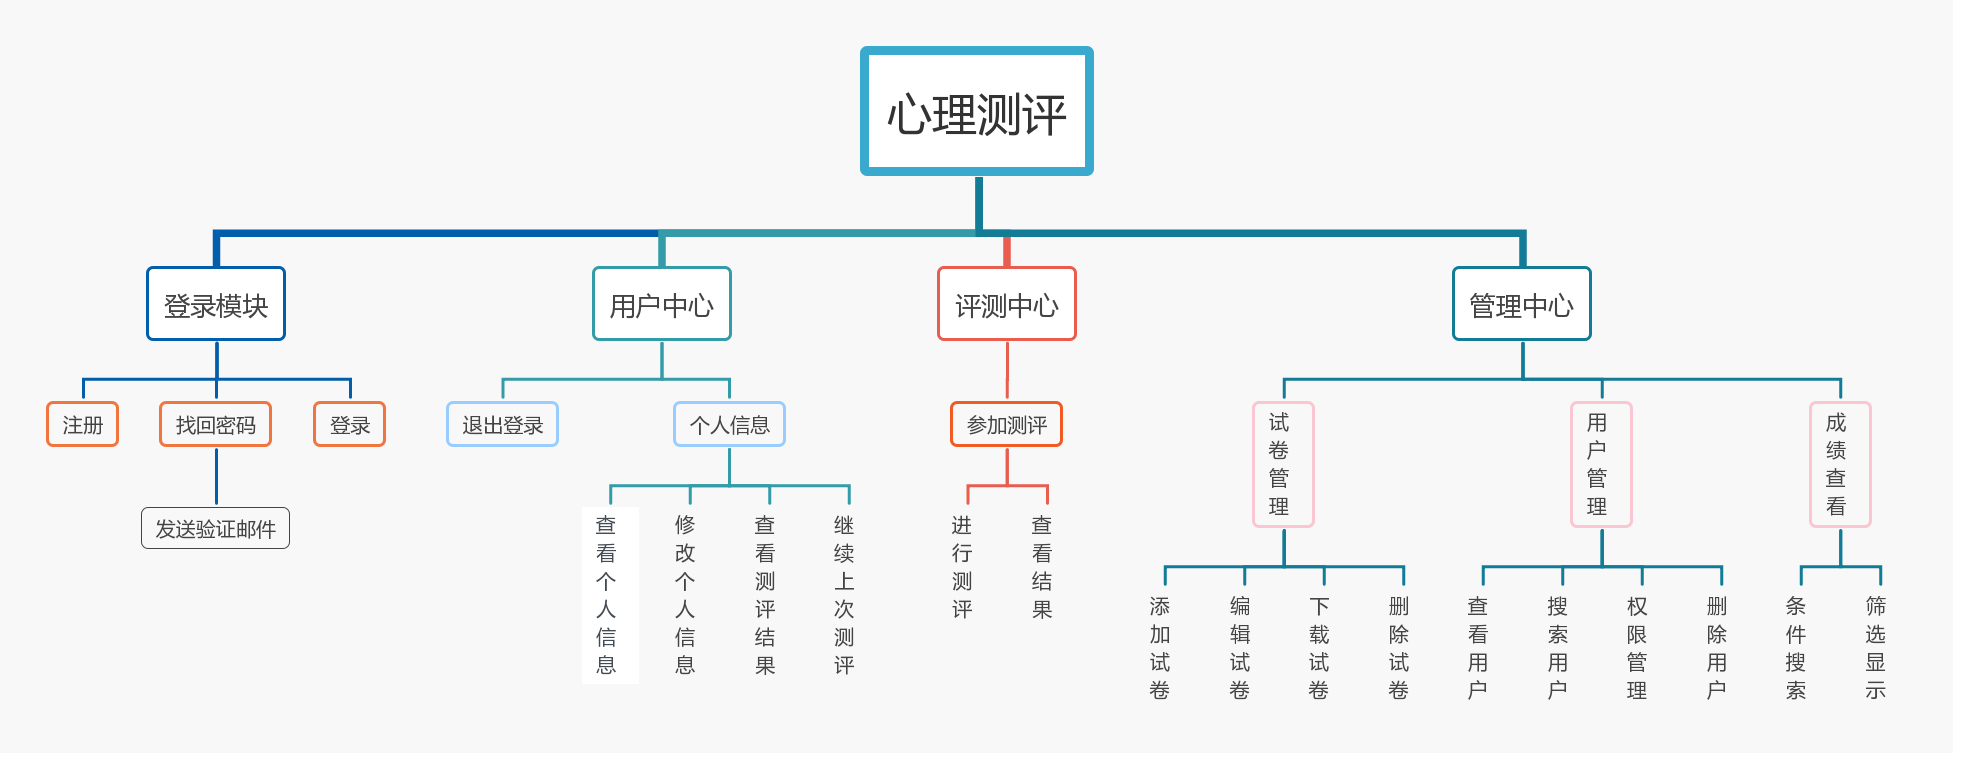
\includegraphics[width=1.0\linewidth]{figure/functions}
	\caption{系统功能设计}
	\label{fig:functions}
\end{figure}

心理评测系统由登陆模块、用户中心、评测中心和管理中心四大模块组成。登陆模块涉及用户的注册、登陆、邮箱验证、找回密码四个功能。用户中心可以修改个人信息、查看已经做的试卷的测评结果、查看未完成试卷的进度。评测中心可以做试卷进行评测和查看结果。管理中心是管理员对试卷、用户、成绩进行管理的模块。

\subsubsection{用例设计}

\begin{figure}[htp]
	\centering
	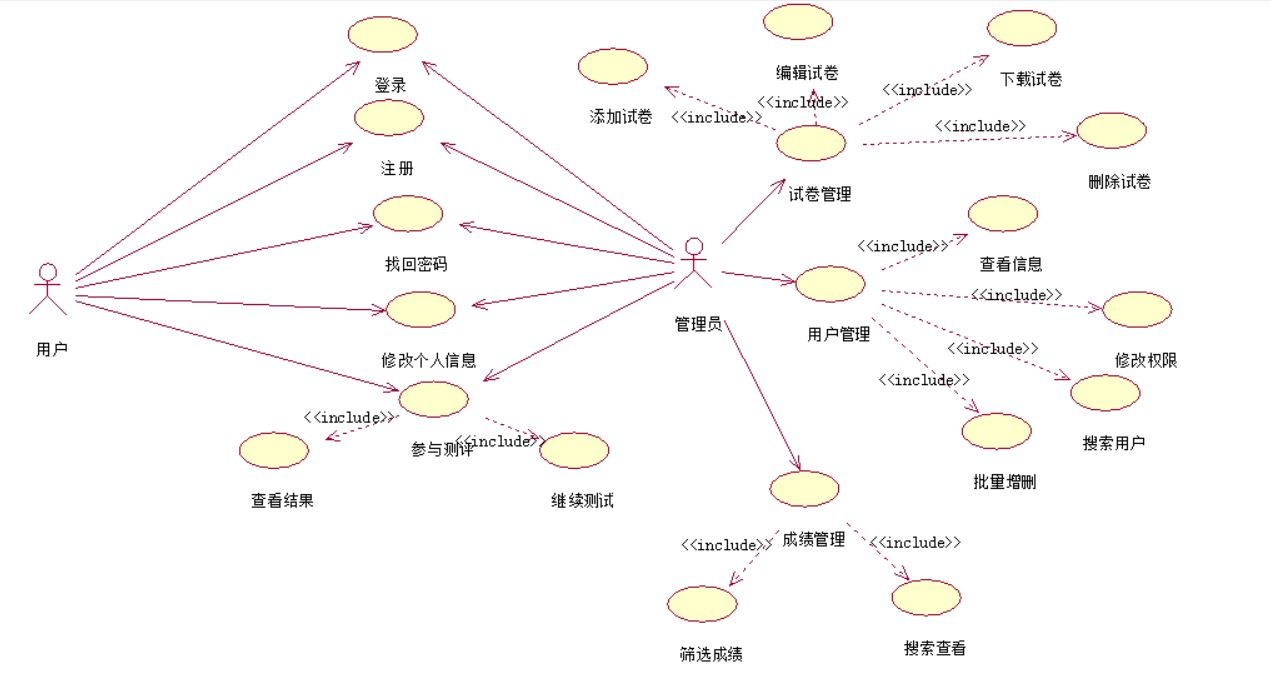
\includegraphics[width=0.8\linewidth]{figure/user_case}
	\caption{系统用例图}
	\label{fig:user_case}
\end{figure}

心里评测系统的用户分为两种类型:用户和管理员,其中管理员可以进行所有用户的操作,并且可以进入管理界面对试卷、用户、成绩进行管理。

\subsubsection{流程设计}

\begin{figure}[thbp!]
	\centering
	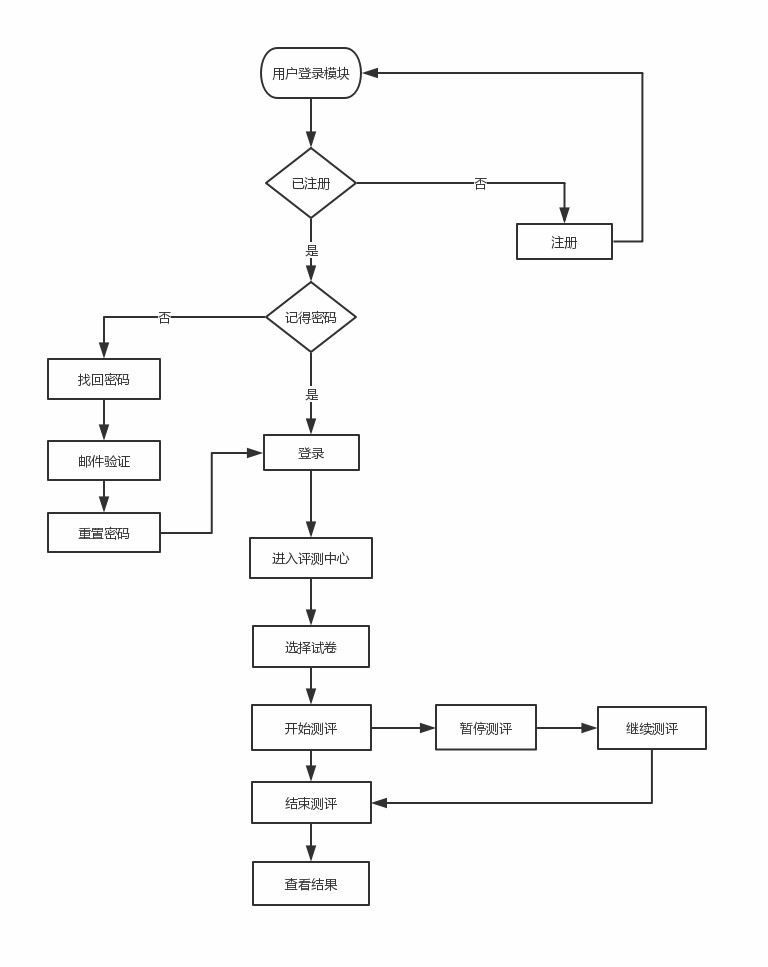
\includegraphics[width=0.8\linewidth]{figure/user_use}
	\caption{用户流程图}
	\label{fig:user_use}
\end{figure}

\begin{figure}[thbp!]
	\centering
	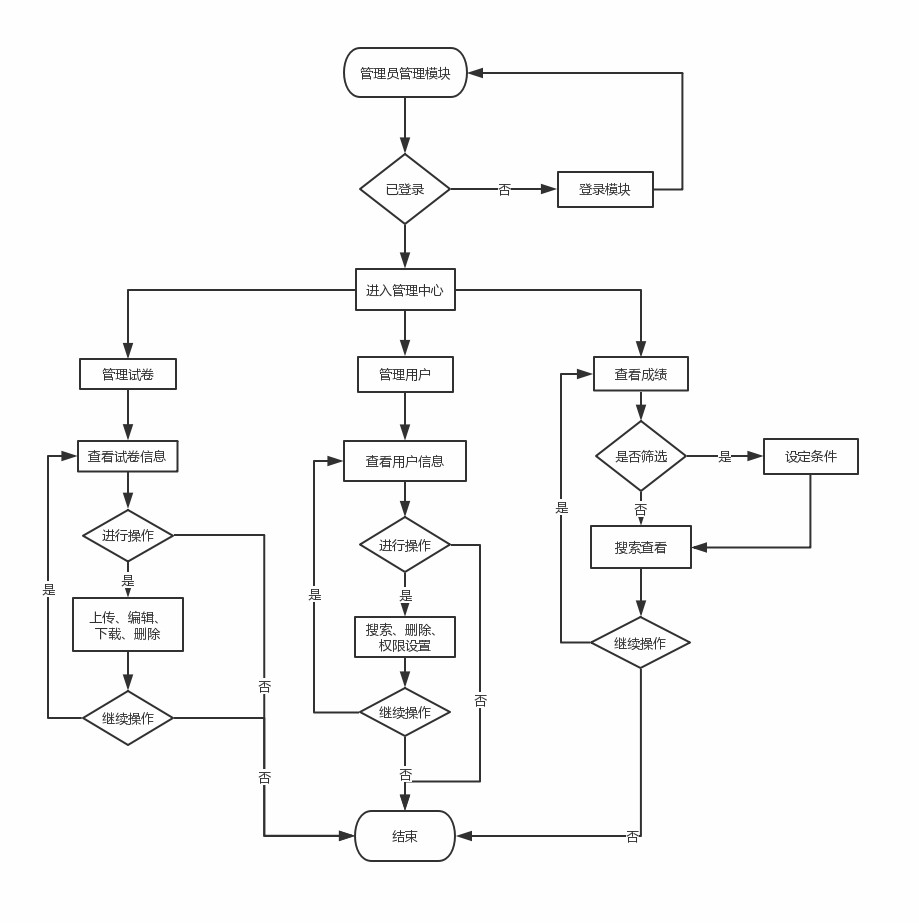
\includegraphics[width=1.0\linewidth]{figure/admin_use}
	\caption{管理员流程图}
	\label{fig:admin_use}
\end{figure}

\subsection{项目设计}

\subsubsection{前端项目架构}

\begin{figure}[thbp!]
	\centering
	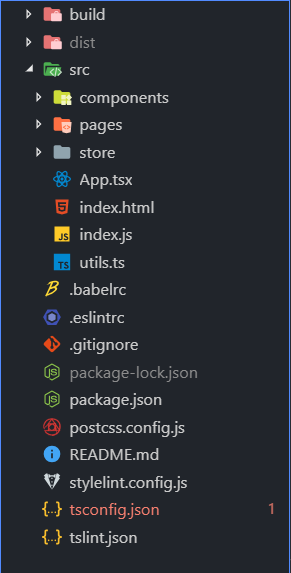
\includegraphics[width=0.3\linewidth]{figure/frontend_structure}
	\caption{前端项目目录}
	\label{fig:frontend_structure}
\end{figure}

build文件夹下存放着webpack的编译打包配置文件,分为两个环境,development开发环境和production生产环境。

dist文件夹是存放着webpack打包后的文件,用作于webpack-dev-server的开发环境文件和上线后的生产环境文件。

src文件夹是项目的根目录,里面的components文件夹存放着公用的组件,pages存放着系统的各个页面文件,store存放着项目所需要用到的redux状态仓库,App.tsx是项目的主页面,index.html是webpack打包注入js依赖的html文件,index.js是项目的主入口,utils.js是项目所需要的共用工具。

.babelrc是babel-loader的配置文件,配置编译js的目标版本。

.eslintrc是eslint代码检查的配置文件。

.gitignore是git仓库push的时候忽略的文件。

package.json是前端项目的架构文件,记载该前端项目所需要的依赖和依赖版本和该前端项目的基本信息。

postcss.config.js是postcss的配置文件。

README.md是描述该项目的markdown文件。

stylelint.config.js是stylelint css代码检查的配置文件。

tsconfig.json是Typescript的编译配置文件。

tslint.json是tslint的配置文件。

\subsubsection{后端项目架构}
\begin{figure}[thbp!]
	\centering
	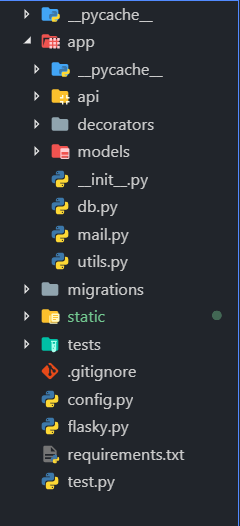
\includegraphics[width=0.3\linewidth]{figure/backend_structure}
	\caption{后端项目目录}
	\label{fig:backend_structure}
\end{figure}

\_\_pycache\_\_是IDE自动生成的sourcemap索引文件夹。

\_\_init\_\_.py文件是该Python包的默认包导出文件。

app文件夹是项目的根目录,api文件夹存放着Resuful API的文件,decorators文件夹存放着项目中所用到的装饰器,models文件夹存放着该项目所用到的所有对应数据库中的数据模型,db.py是该项目连接数据库获得数据库实例的文件,mail.py是该项目所使用到的邮箱模块,utils.py是该项目的工具库。

migrations是Flask-Migrate根据Sqlalchemy ORM数据模型定义进行数据库备份的文件夹。

static是该后端项目的静态文件存放目录。

tests是后端项目的测试文件存放目录。

.gitignore是git仓库索要忽略文件的声明文件。

config.py是该项目的配置文件。

flasky.py是该项目的主入口文件,启动文件。

requirements.txt记录着该项目的依赖和依赖版本。

\subsection{项目重要依赖}

\subsubsection{React}

React是一个声明式,组件化的前端框架。其使用Virtual DOM技术把应用状态和DOM分离开来,搭配Diff算法来最小颗粒的更新DOM,而这一切开发者都不需要关心,开发者只需要专注注意力在开发业务代码上。React拥有极丰富的生态,本项目中还使用了React-redux来进行redux状态仓库的管理。

\begin{lstlisting}[language=C]
class App extends Component {
  public componentDidMount() {
  	...
  }
  
  public render() {
	return (
	  <div>
	    this is App
	      <a onClick={this.onClick}>
	  </div>
	)
  }
	  
  private onClick = (e: ClickEvent) => {
    e.preventDefault();
    ...
  }
}
\end{lstlisting}

\begin{center}
	{\small React编写组件}
\end{center}

所有React组件都要继承React.Component,拥有React组件的生命周期,每个React组件需要实现一个继承父类的render方法,来控制组件如何进行渲染。

\subsubsection{Flask}

Flask是一个使用 Python 编写的轻量级 Web 应用框架。其 WSGI 工具箱采用 Werkzeug ,模板引擎则使用 Jinja2 。Flask使用 BSD 授权。Flask也被称为 “microframework” ,因为它使用简单的核心,用 extension 增加其他功能。Flask没有默认使用的数据库、窗体验证工具。本项目中使用了Flask-Migrate来进行数据库的备份,Flask-Mail来进行邮件的发送,Flask-SqlAlchemy来进行更加简单的操作SqlAlchemy。

\begin{lstlisting}[language=C]
@app.route("/index")
def Index():
	return "<h1>Hello, Index</h1>"
\end{lstlisting}

\begin{center}
	{\small Flask定义视图路由}
\end{center}

传给app.route的是一个路径字符串,该方法返回一个装饰器,装饰器装饰路由函数,每个路由函数返回一个页面或者数据。

\subsubsection{Typescript和Javascript}

项目使用的前端语言并非常规的Javascript而是它的超集——Typescript,其作为超集在绝对兼容Javascript代码的前提下,加入了许多静态语言所拥有的特性,比如接口、泛型、类型判断等等。Javascript作为脚本语言其灵活性和方便性为大家所称道,但是也由于其灵活性,前端代码的质量低下导致项目难以维护和扩展,Typescript就是解决Javascript严谨性而诞生的一门语言。Java作为世界上用途最广泛,使用人数最多的语言就是因为其严谨性得到了很多企业的偏爱,Typescript看起来80\%都和Java很相似,可以理解为在Javascript的基础上加了一层代码检查和提示。

\subsubsection{前端构建工具——Webpack}

浏览器的版本众多,浏览器与浏览器之间的内核有许多差异,这导致同一份代码可能在不同浏览器下的表现不同,通过人工的方式编写兼容代码会有很高的人力成本和时间成本。同时在以前的开发过程中,前端依赖后端导致前端开发与后端严重耦合,降低了开发效率。前端工程化时代的到来,让前端拥有自己的项目构建能力,同时还解决了不同浏览器之间的兼容问题,诞生了许多前端构件工具,Gul、Grunt、Webpack等等。其中Webpack是当下活跃度最高,最火热的前端构建工具。

Webpack最主要的两个功能是编译和打包。本项目所使用的React是使用JSX语法,不是浏览器默认可支持的语法,所以要将我们的前端代码编译成浏览器可识别的代码。Webpack最重要的两个概念就是loader和plugin,loader负责各种类型文件(.css,.js,.ts,.png......)的编译工作,可以将他们转化成目标浏览器的可识别文件,plugin则负责除了编译以外的所有工作,包括打包,体积优化,分离依赖等等。

\begin{lstlisting}[language=C]
{
  test: /\.jsx?$/,
  exclude: /node_modules/,
  use: ["babel-loader"]
},
{
  test: /\.tsx?$/,
  exclude: /node_modules/,
  use: [{
    loader: "ts-loader",
    options: {
      transpileOnly: true,
      getCustomTransformers: () => ({
          before: [
            require("ts-import-plugin")({
              libraryName: "antd",
              libraryDirectory: "es",
              style: "css"})
          ]
      }),
      compilerOptions: { module: "es2015" }
    }
  }]
}
\end{lstlisting}

\begin{center}
	{\small Webpack编译jsx和tsx文件成es5的配置}
\end{center}

Webpack还提供了前端可实时预览的热更新服务器————webpack-dev-server,该插件可以实时的检测项目文件的变化并重新编译和打包让浏览器的页面刷新。

Webpack打包体积优化也是一个深奥的学问。

Webpack在原始配置的情况下,因为是单页面应用,所以打包出来以后的bundle文件非常之大,高达4MB,这对于首屏加载是非常不利的,过长的白屏会流失很多的用户量,所以Webpack的优化也是一门学问。

常用的优化有以下几点:

(1) 配置optimization中的splitChunks选项,会根据依赖图对于多次依赖的包单独打包然后进行引用。

(2) 配置externals选项对于第三库在html文件中进行CDN引用,打包时候忽略该库。

(3) 使用uglifyjsPlugin对打包文件进行压缩。

(4) 使用懒加载进行加载组件和页面,react-loadable可以通过一个高阶组件包裹我们的异步组件使用import函数进行异步的加载组件,当加载成功的时候显示组件否则就加载Loading组件。

(5) 配置Gzip。

进行上面的优化以后,打包以后的文件按照路由和组件分成了十几个文件,最大的体积不超过400KB,减少了首屏加载的时间。

\subsubsection{Pandas}

Pandas是一个数据科学分析第三方库,可以方便的建立矩阵以及对矩阵中的数据进行各种数学运算和变换,在解析试卷和成绩分析的时候有很多使用。同时可以对矩阵中的数据进行清理和类型的转换。

\subsection{数据库设计}

通过SqlAlchemy我们可以方便的在数据库中创建一个表并生成记录,同时也可以方便的进行数据库操作,定义数据之间的关系,搭配Flask-Migrate还可以方便的进行数据库备份、恢复和回滚。

这个系统的主要有三个表,用户表(users),试卷表(papers),成绩表(grades),数据库实体之间的关系,箭头都代表一对多关系,粗体字体为必填字段。

\begin{figure}[thbp!]
	\centering
	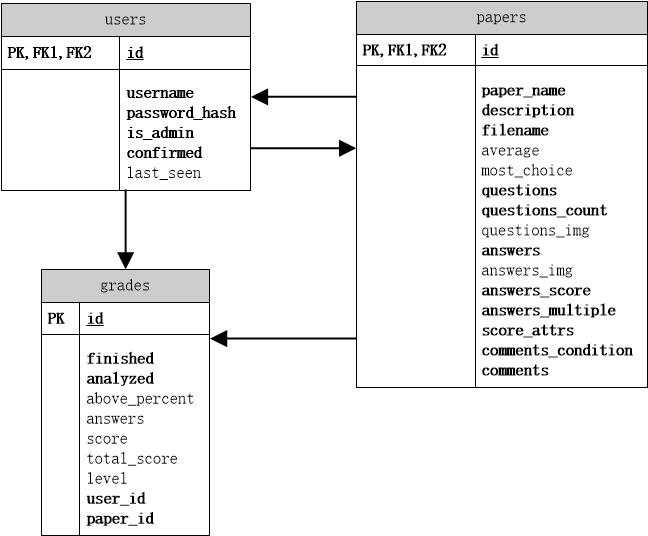
\includegraphics[width=0.7\linewidth]{figure/entity_relationship}
	\caption{数据库关系}
	\label{fig:entity_relationship}
\end{figure}

\subsubsection{一对多关系}

如图中,用户表和成绩表,试卷表和成绩表之间都为一对多关系。SqlAlchemy中可以方便的通过relationship和foreignKey进行设置一对多关系。

\begin{lstlisting}[language=C]
class User(Model):
...
grades = relationship("Grade", backref="user", lazy="dynamic",
cascade="all, delete-orphan", passive_deletes=True)

class Paper(Model):
...
grades = relationship("Grade", backref="paper", lazy="dynamic",
cascade="all, delete-orphan", passive_deletes=True)

class Grade(Model):
...
user_id = Column(Integer, ForeignKey("users.id",
ondelete="CASCADE"))
paper_id = Column(Integer, ForeignKey("papers.id",
ondelete="CASCADE"))
\end{lstlisting}

\begin{center}
	{\small 建立用户和成绩,试卷与成绩之间的一对多关系}
\end{center}

relationship的这一端代表着1的这一端,backref传入的是在Grade对象下如何访问User或者Paper对象,lazy代表如何访问这个对象,一对多之间的关系通过外键的形式进行设置,比如users.id代表着是users这张表中的id作为外键。同时外键的字段设置需要和做外键的字段类型一模一样,否则会报错。

(1) select,默认选项,直接查找出所有对象,例如user.grades直接通过列表列出所有该用户下的grade

(2) dynamic返回的是一个查询集,例如 users.grades.filter\_by(...)返回的是一个查询集可以进行筛选操作。

(3) joine类似于select,但是seletc在查询的过程中需要查询两个表,而joined是建立一个新的连结表进行查询,在数额大的情况下使用joined能节省不少性能。

\begin{center}
	{\small lazy选项}
\end{center}

SqlAlchemy作为最强大的ORM工具当然不只是定义关系,还有就是定义实体不存在的时候如何处理与其相关的数据,加入一个用户被删除了,那么于其关联的成绩也应该要全部删除,而不是作为冗余数据存在数据库中,一套试卷被删除了同理。那么cascade就是干这个事情的。

(1) save-update,默认选项,添加一条数据的时候会把其他和它相关的数据都添加到数据库中。

(2) merge,默认选项,合并一个对象的时候会将使用了relationship相关联的对象也进行merge操作。

(3) expunge,移除操作的时候,会将相关联的对象也进行移除,这个操作只是从session中删除,而不是从真正的数据库中删除。

(4) all,包含上面所有的选项。

(5) delete-orphan,删除相关的孤儿数据。

\begin{center}
	{\small cascade选项}
\end{center}

对应的要在多的那一端设置ondelete属性。

至此一对多的关系就设置好了,使用Flask-Migrate升级数据库的时候可以自动检测相关外键的设置然后更新数据库。

\subsubsection{多对多关系}

\begin{figure}[thbp!]
	\centering
	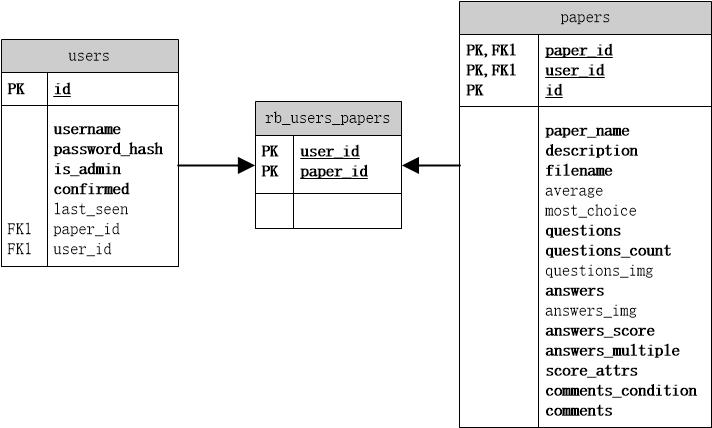
\includegraphics[width=1.0\linewidth]{figure/rb_users_papers}
	\caption{多对多关系}
	\label{fig:rb_users_papers}
\end{figure}

一个用户可以做多张试卷,一张试卷也可以有很多用户来做。这就是一个多对多关系。多对多关系中,需要一个额外的连接表来做查询。

\begin{lstlisting}[language=C]
class User(Model):
...
papers = relationship("Paper", secondary=rb_users_papers,
lazy="dynamic")

class Paper(Model):
...
users = relationship("User", secondary=rb_users_papers,
lazy="dynamic")

// 连接表
rb_users_papers = Table(
"rb_users_papers",
Column("user_id", Integer, ForeignKey("users.id"),
primary_key=True),
Column("paper_id", Integer, ForeignKey("papers.id"),
primary_key=True)
)
\end{lstlisting}

\begin{center}
	{\small 多对多关系代码}
\end{center}

上面的代码说明了users表和papers表之间是通过一个rb\_users\_papers进行连接查询的,同时连接表中的每个字段都需要与原字段的属性相同。在原表中的relationship中需要设置secondary属性来进行使用连接表的查询。使用连接表进行连接的两个表,任何一条记录被删除以后相关的连接表记录也会被删除,当然也可以设置与其关联的记录也被删除,但在此处的情况不适合这样做,试想一下,如果一个用户记录被删除了,那么该用户做过所有的试卷记录也会被删除,别人就无法做了,这样是非常的不合适的情况。

数据库的设计是一个完善的软件系统必备也是最重要的一个阶段,一个好的数据库设计能让一个系统的性能良好、易于维护、易于拓展。有些人可能会觉得直接手写sql更加灵活和方便,但是如果作为一个多人维护开发的系统来说,每个人都有自己写sql的习惯,会让项目代码水平层次不齐难于维护,这时候就要使用SqlAlchemy这种工具了,通过一种OOP的方式来进行数据库的管理。